%%%%%%%%%%%%%%%%%%%%%%%%%%%%%%%%%%%%%%%%%
% fphw Assignment
% LaTeX Template
% Version 1.0 (27/04/2019)
%
% This template originates from:
% https://www.LaTeXTemplates.com
%
% Authors:
% Class by Felipe Portales-Oliva (f.portales.oliva@gmail.com) with template 
% content and modifications by Vel (vel@LaTeXTemplates.com)
%
% Template (this file) License:
% CC BY-NC-SA 3.0 (http://creativecommons.org/licenses/by-nc-sa/3.0/)
%
%%%%%%%%%%%%%%%%%%%%%%%%%%%%%%%%%%%%%%%%%

%----------------------------------------------------------------------------------------
%	PACKAGES AND OTHER DOCUMENT CONFIGURATIONS
%----------------------------------------------------------------------------------------

\documentclass[
	french,
	11pt, % Default font size, values between 10pt-12pt are allowed
	%letterpaper, % Uncomment for US letter paper size
	%spanish, % Uncomment for Spanish
]{fphw}

% Template-specific packages
\usepackage{babel}
\usepackage[utf8]{inputenc} % Required for inputting international characters
\usepackage[T1]{fontenc} % Output font encoding for international characters
\usepackage{mathpazo} % Use the Palatino font
% \usepackage{iwona} % Use the Iwona font

\usepackage{amsmath}
\usepackage{mathtools}
\usepackage{xfrac} 

\usepackage{graphicx} % Required for including images
\usepackage[textfont=it]{caption}  %% To manage long captions in images
\usepackage{subcaption}
\captionsetup{justification=centering}

\usepackage{float}
\graphicspath{ {./img/} }

\usepackage{booktabs} % Required for better horizontal rules in tables

\usepackage{listings} % Required for insertion of code

\usepackage{array} % Required for spacing in tabular environment

\usepackage{enumerate} % To modify the enumerate environment

\usepackage{amssymb}
\usepackage{enumitem}	%% % To modify the itemize bullet character

\usepackage{xcolor}
\usepackage{listings}
\colorlet{mygray}{black!30}
\colorlet{mygreen}{green!60!blue}
\colorlet{mymauve}{red!60!blue}
\lstset{
  backgroundcolor=\color{gray!10},  
  basicstyle=\scriptsize\ttfamily,
  columns=fullflexible,
  breakatwhitespace=false,      
  breaklines=true,                
  captionpos=b,                    
  commentstyle=\color{mygreen}, 
  extendedchars=true,              
  frame=single,                   
  keepspaces=true,             
  keywordstyle=\color{blue},      
  language=c++,                 
  numbers=none,                
  numbersep=5pt,                   
  numberstyle=\tiny\color{blue}, 
  rulecolor=\color{mygray},        
  showspaces=false,               
  showtabs=false,                 
  stepnumber=5,                  
  stringstyle=\color{mymauve},    
  tabsize=3,                      
  title=\lstname                
}

\usepackage[linkcolor=blue,colorlinks=true]{hyperref}
\usepackage{cleveref}
\usepackage{siunitx}
\newcommand{\bvec}[1]{\bm{#1}}    %% For vector notation
\newcommand{\myvec}[3]{\begin{pmatrix} #1  \\ #2 \\ #3 \end{pmatrix}}   %% vecteur 3d
\newcommand{\mymat}[9]{\begin{pmatrix} #1 & #2 & #3 \\ #4 & #5 & #6 \\ #7 & #8 &#9 \end{pmatrix}}  %% Matrice 3*3

\renewcommand{\vector}[4]{\begin{pmatrix} #1  \\ #2 \\ #3 \\ #4 \end{pmatrix}}   %% vecteur 3d
% \newcommand{\mymatrix}[16]{\begin{pmatrix} #1 & #2 & #3 & #4 \\ #4 & #6 & #7 & #8 \\ #9 & #10 & #11 & #12 \\ #13 & #14 & #15 & #16 \end{pmatrix}}  %% Matrice 3*3

\setlength\parindent{0pt}

\newcommand{\hquad}{\hspace{0.5em}} %% Bew command for half quad
% \setlength\parindent{0pt}	%% To remove all indentations

%----------------------------------------------------------------------------------------
%	ASSIGNMENT INFORMATION
%----------------------------------------------------------------------------------------

\title{TP \#3} % Assignment title

\author{Roussel Desmond Nzoyem} % Student name

\date{\today} % Due date

\institute{Université de Strasbourg \\ UFR de Mathématiques et Informatique} % Institute or school name

\class{EDP 2} % Course or class name

\professor{Pr. Philippe Helluy} % Professor or teacher in charge of the assignment

%----------------------------------------------------------------------------------------

\begin{document}

\maketitle % Output the assignment title, created automatically using the information in the custom commands above

%----------------------------------------------------------------------------------------
%	ASSIGNMENT CONTENT - SECTION 1
%----------------------------------------------------------------------------------------


\section*{Résolution numérique du système de Saint-Venant en deux dimensions}

Le modèle de Saint-Venant en deux dimensions s'écrit 

\begin{align*}
	\partial_t w + \partial_x (hu) + \partial_y(hv)  &=0 \\
	\partial_t(hu) + \partial_x \left(hu^2 + g\frac{h^2}{2} \right) + \partial_y(huv) &= -gh \partial_x A \tag{$\mathcal{S}$}\\ 
	\partial_t(hv) + \partial_x(huv) + \partial_y \left(hv^2 + g\frac{h^2}{2} \right) &= -gh \partial_y A 
	\label{eq:stVenant2D}
\end{align*}

où 
\begin{itemize}
	\item $A(x,y)$ désigne l'altitude du point $(x,y)$
	\item $h(x,y,t) \geq 0$ désigne la hauteur du point $(x,y)$ à l'instant $t$
	\item $u(x,y,t)$ désigne la composante suivant $x$ du vecteur vitesse au point $(x,y)$ à l'instant $t$
	\item $v(x,y,t)$ désigne la composante suivant $y$ du vecteur vitesse au point $(x,y)$ à l'instant $t$
\end{itemize}


Notre domaine d'étude sera le carré $[0,L]\times[0,L]$ tel que la hauteur d’eau $h$ soit petite devant $L$.


%----------------------------------------------------------------------
\subsection*{Question 1.}

\begin{problem}
Écriture du système de Saint-Venant 2D sous la forme 
\begin{equation}
	\partial_t w + \partial_x f_1(w) + \partial_y f_2(w) = S(w) \tag{$\mathcal{S}'$}	
\end{equation}
\end{problem}


\subsection*{Réponse} 

On introduit $A$ comme une variable indépendante du temps i.e $\partial_t A = 0$ et on considère la variable conservative 
$$w= \vector{w_1}{w_2}{w_3}{w_4} = \vector{h}{hu}{hv}{A}$$
On remarque que le système $(\mathcal{S})$ se met facilement sous la forme
$$
\partial_t w + \partial_x f_1(h,u,v,A) + \partial_y f_2(h,u,v,A) = S(h,u,v,A)
$$
où les fonctions $f_1$, $f_2$, et $S$ sont exprimées en termes de variables primitives $h, u$, $v$ et $A$. 
$$f_1(h,u,v,A) = \vector{hu}{hu^2 + \dfrac{gh^2}{2}}{huv}{0}, \qquad f_2(h,u,v,A) = \myvec{hv}{huv}{hv^2 + \dfrac{gh^2}{2}{}}, \qquad S(h,u,v,A) = \vector{0}{-gh\partial_xA}{-gh\partial_y A}{0}$$
En supposant $w_1>0$, on les exprime en fonction de $w$ en remarque que $$\vector{h}{u}{v}{A} = \vector{w_1}{\sfrac{w_2}{w_1}}{\sfrac{w_3}{w_1}}{w_4}$$
Le système $(\mathcal{S})$ se met sous la forme $(\mathcal{S}')$ demandée avec 
$$f_1(w) = \vector{w_2}{\sfrac{w_2^2}{w_1} + \sfrac{gw_1^2}{2}}{\sfrac{w_2w_3}{w_1}}{0}, \qquad f_2(w) = \vector{w_3}{\sfrac{w_2w_3}{w_1}}{\sfrac{w_3^2}{w_1} + \sfrac{gw_1^2}{2}}{0}, \qquad S(w)=\vector{0}{-gh\partial_x w_4}{-gh\partial_x w_4}{0}$$



%----------------------------------------------------------------------
\subsection*{Question 2.}

\begin{problem}
Vérifions que le système de Saint-Venant 2D est hyperbolique.
\end{problem}


\subsection*{Réponse} 
Pour cela, posons $n=(n_1,n_2)$ et $f(w)\cdot n = f_1(w)n_1 + f_2(w)n_2$ et vérifions que la matrice jacobienne de la divergence du flux $B = \partial_w \left( f(w)\cdot n \right)$ est diagonalisable pour tout $w$ tel que $w_1 \geq 0$ et pour tout $n$. 

\noindent En remarquant que les équations sont invariantes par rotation (aucune direction de propagation n'est privilégiée), il suffit de regarder l'hyperbolicité dans une direction. Prenons donc $n=(1,0)$ et étudions les valeurs propres de $B$. On a, pour $w_1 > 0$,
$$f(w)\cdot n = f_1(w) = \vector{w_2}{\frac{w_2^2}{w_1} + \frac{gw_1^2}{2}}{\frac{w_2w_3}{w_1}}{0}$$
et 
% \mymat{0}{1}{0}{+gw_1+gA}{\dfrac{2w_2}{w_1}}{0}{-\dfrac{w_2w_3}{w_1}}{\dfrac{w_3}{w_1}}{\dfrac{w_2}{w_1}}
\begin{align*}
	B = \partial_w \left( f(w)\cdot n \right) = \begin{pmatrix} 0 & 1 & 0 & 0 \\ \frac{w_2^2}{w_1^2}+gw_1 & \frac{2w_2}{w_1} & 0 & 0 \\ -\frac{w_2w_3}{w_1} & \frac{w_3}{w_1} & \frac{w_2}{w_1} & 0 \\ 0 & 0 & 0 & 0 \end{pmatrix}
\end{align*}
et donc pour tout $\lambda \in \mathbb{R} $,
\begin{align*}
	\text{det}(B-\lambda I_3) &= \text{det} \begin{pmatrix} -\lambda & 1 & 0 & 0 \\ \frac{w_2^2}{w_1^2}+gw_1 & \frac{2w_2}{w_1}-\lambda & 0 & 0 \\ -\frac{w_2w_3}{w_1} & \frac{w_3}{w_1} & \frac{w_2}{w_1}-\lambda & 0 \\ 0 & 0 & 0 & -\lambda \end{pmatrix}  \\
	&= -\lambda \left[ -\lambda \left( \frac{2w_2}{w_1} -\lambda \right)\left( \frac{w_2}{w_1} -\lambda \right) + \left( \frac{w_2^2}{w_1^2} +gw_1 \right)\left( \frac{w_2}{w_1} -\lambda \right) \right]    \\
	&= -\lambda \left( \frac{w_2}{w_1} -\lambda \right) \left[ \lambda^2 - \lambda \left(\frac{2w_2}{w_1}\right) + \frac{w_2^2}{w_1^2}-gw_1  \right] \\
	&= -\lambda \left( \frac{w_2}{w_1} -\lambda \right) \left( \frac{w_2}{w_1} - \sqrt{gw_1} \right) \left( \frac{w_2}{w_1} + \sqrt{gw_1} \right)
\end{align*}
On constate donc que $B$ admets trois valeurs propres réelles (pas forcément ordonnées et pas forcément distinctes) définies par 
\begin{align*}
	\lambda_1(w,n) &= \frac{w_2}{w_1} - \sqrt{gw_1 } \\
	\lambda_2(w,n) &= 0 \\
	\lambda_3(w,n) &= \frac{w_2}{w_1} \\
	\lambda_4(w,n) &= \frac{w_2}{w_1} + \sqrt{gw_1}
\end{align*}
Ce calcul se généralise à toutes les directions $n$ de l'espace. On montre, en repassant aux variables primitives et en posant $U = (u,v)$, que 
\begin{align*}
	\lambda_1(w,n) &= U\cdot n - \sqrt{gh} \\
	\lambda_2(w,n) &= 0 \\
	\lambda_3(w,n) &= U\cdot n \\
	\lambda_4(w,n) &= U\cdot n + \sqrt{gh}
\end{align*}
valable pour tout $w$ tel que $w_1 \geq 0$ \footnote{Le cas $w_1 = 0$ i.e. $h=0$ tolérant les zones sèches nécessite un traitement particulier, qu'on pourra résoudre en travaillant avec les variables primitives.}. Le polynôme caractéristique de $B$ est scindé à valeurs propres réelles (et donc diagonalisable). Le système ($\mathcal{S}$) de Saint-Venant 2D est donc hyperbolique.


%----------------------------------------------------------------------
\subsection*{Question 3.}

\begin{problem}
	Expression du flux numérique $f(w_L, w_R, n)$ de Rusanov en 2D en vue d'une approximation numérique du système de Saint-Venant.
\end{problem}


\subsection*{Réponse} 
En s'inspirant de la définition du flux de Rusanov en 1D, on écrit
\begin{align*}
	f(w_L, w_R, n) = \frac{1}{2}\left( f(w_L,n)+f(w_R,n)  \right) - \frac{\lambda_{LR}}{2}(w_R - w_L)
\end{align*}
où la vitesse de Rusanov locale satisfait la condition suivante\footnote{Remarquons que seules les 3 premières variables conservatives $w_1,w_2,$ et $w_3$ (et donc 3 valeurs propres $\lambda_1, \lambda_3,$ et $\lambda_4$) seront généralement considérées. Ceci correspondra généralement à un fond plat nul, i.e $A(\cdot,\cdot)=0$. } 
$$
\lambda_{LR} \geq \max_{k=1,2,3}{\big\{ \max{ \big\{ \vert \lambda_k(w_L,n) \vert, \, \vert \lambda_k(w_R,n) \vert }\big\} \big\}}
$$
on choisit donc 
$$
\lambda_{LR} = \max{ \Big\{ \vert U_L\cdot n \vert + \sqrt{gh_L}, \,\, \vert U_R\cdot n \vert + \sqrt{gh_R} }\Big\}
$$
À l'intérieur du Kernel de calcul OpenCL utilisé pour les simulations, le flux de Rusanov s'implémente comme ceci:
\begin{lstlisting}[language=C, caption={Flux numérique de Rusanov en 2D},breaklines]
void flux_rusa_2d(float *wL, float *wR, float* vnorm, float* flux){
	float fL[_M];
	float fR[_M];
	
	fluxphy(wL, vnorm, fL);
	fluxphy(wR, vnorm, fR);
	
	float UL[2] = {wL[1]/wL[0], wL[2]/wL[0]};
	float UR[2] = {wR[1]/wR[0], wR[2]/wR[0]};
	
	float cL = sqrt(_G*wL[0]);
	float cR = sqrt(_G*wR[0]);
	
	float lambdaL = cL;
	float lambdaR = cR;
	for (int i=0; i<2; i++){
		lambdaL += fabs(UL[i]*vnorm[i]);
		lambdaL += fabs(UR[i]*vnorm[i]);
	}
	
	float MyLAMBDA = lambdaL>lambdaR?lambdaL:lambdaR;
	for(int iv = 0; iv < _M; iv++)
		flux[iv] = 0.5f * (fL[iv] + fR[iv]) - 0.5f * MyLAMBDA * (wR[iv] - wL[iv]); 
}
\end{lstlisting}

\noindent Quelque résultats sont présentés aux \cref{fig:Rusa1,fig:Rusa2,fig:Rusa3}. Ils correspondent tous à une rupture totale de barrage à l'instant initial. La forme du barrage et le fond pourront varier d'une simulation à l'autre, mais toutes les simulations que nous traiterons dans ce rapport auront les paramètres suivants \footnote{Ces mêmes paramètres seront utilisés dans les autres sections du rapport.}: 
\begin{itemize}
	\item Domaine de taille $[0,L]\times[0,L] = [0,1]\times[0,1]$
	\item Nombre de mailles suivant $x$: $N_x = 1024$
	\item Nombre de mailles suivant $y$: $N_y = 1024$
	\item Temps maximal (final) de simulation: $t_{max} = 0.05$ \textit{(sauf indication contraire)}.
	\item Coefficient $CFL = 0.8$. Il est choisi tel que $\Delta t = CFL \times \dfrac{\Delta x \Delta y}{2(\Delta x + \Delta y)\left( u_{max} + \sqrt{gh_{max}} \right)}$ à chaque itération ($h_{max}$ et $u_{max}$ désignant respectivement les valeurs maximales de la hauteur d'eau et de l'intensité du vecteur vitesse durant toute la simulation).
	\item La vitesse d'eau initiale sur tout le domaine $(u,v) = (0,0)$
	\item La hauteur d'eau initiale à l'intérieur du barrage $h=2$, et à l'extérieur du barrage $h=1$. 
	\item Le fond du domaine sera plat d'altitude nulle i.e $A(x,y)=0 \hquad \forall \, (x,y)\in[0,L]\times[0,L]$ \textit{(sauf indication contraire)}.
\end{itemize} 

\begin{figure}[H]
	\centering
	\begin{subfigure}{0.32\textwidth}
		\centering
		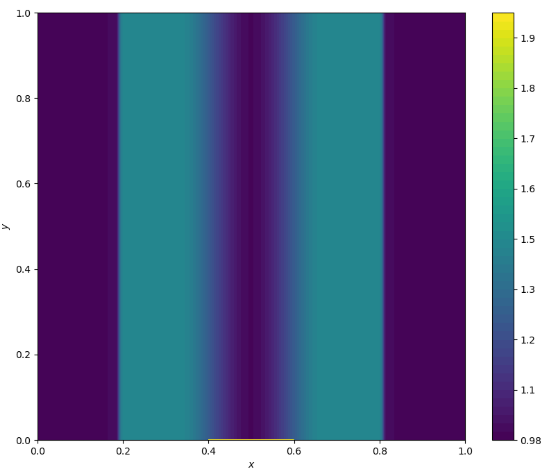
\includegraphics[width=\textwidth,height=0.85\textwidth]{Rusa1h.png}
		\caption{Hauteur d'eau}
		\label{fig:Rusa1h}
	\end{subfigure}
	\begin{subfigure}{0.32\textwidth}
		\centering
		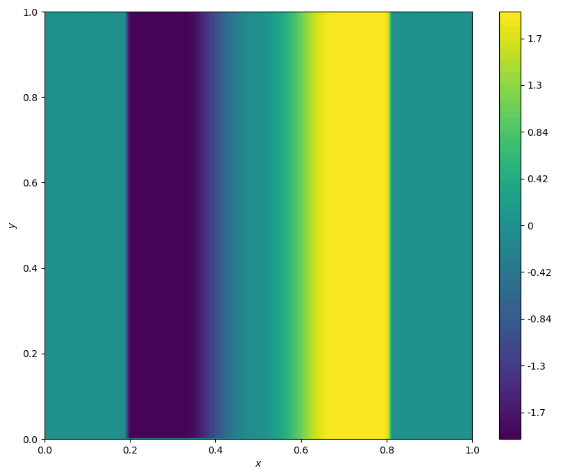
\includegraphics[width=\textwidth,height=0.85\textwidth]{Rusa1u.png}
		\caption{Vitesse suivant $x$}
		\label{fig:Rusa1u}
	\end{subfigure}
	\begin{subfigure}{0.32\textwidth}
		\centering
		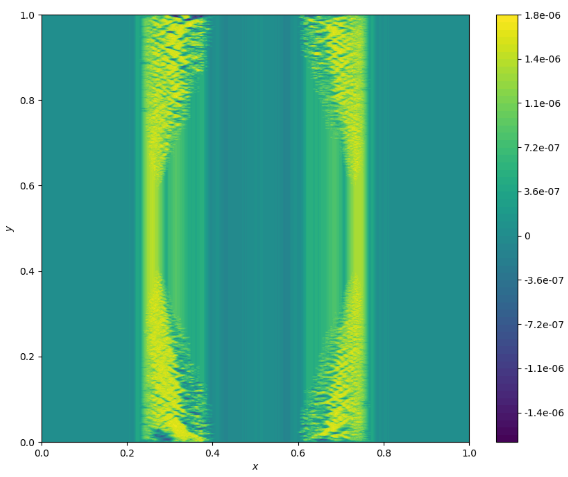
\includegraphics[width=\textwidth,height=0.85\textwidth]{Rusa1v.png}
		\caption{Vitesse suivant $y$}
		\label{fig:Rusa1v}
	\end{subfigure}
	\caption{Illustration de la résolution du système de Saint-Venant par le flux de Rusanov 2D. La condition initiale imposée est  $ h = 2$ pour $ 0.4 \leq x \leq 0.6$.}
	\label{fig:Rusa1}
\end{figure}

\begin{figure}[H]
	\centering
	\begin{subfigure}{0.32\textwidth}
		\centering
		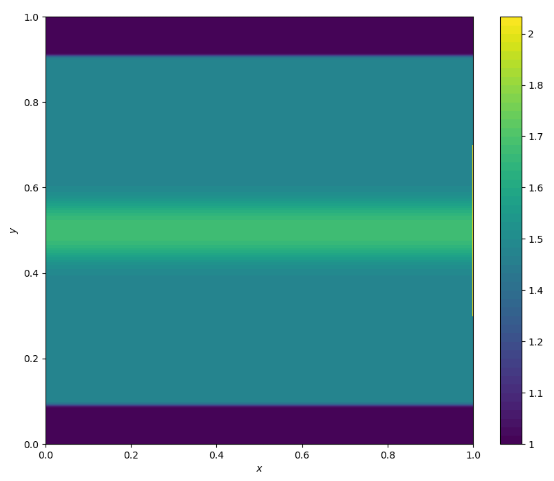
\includegraphics[width=\textwidth,height=0.85\textwidth]{Rusa2h.png}
		\caption{Hauteur d'eau}
		\label{fig:Rusa2h}
	\end{subfigure}
	\begin{subfigure}{0.32\textwidth}
		\centering
		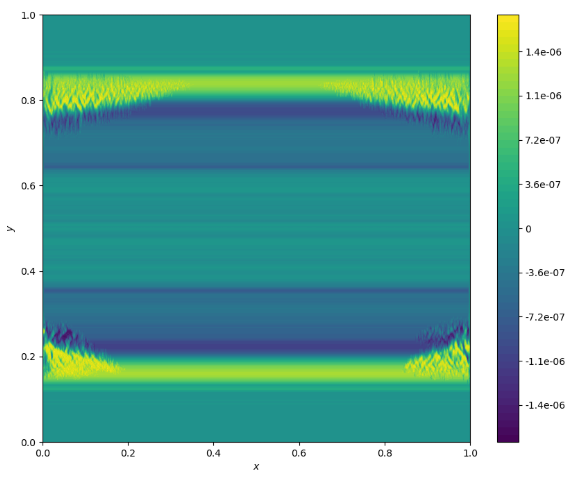
\includegraphics[width=\textwidth,height=0.85\textwidth]{Rusa2u.png}
		\caption{Vitesse suivant $x$}
		\label{fig:Rusa2u}
	\end{subfigure}
	\begin{subfigure}{0.32\textwidth}
		\centering
		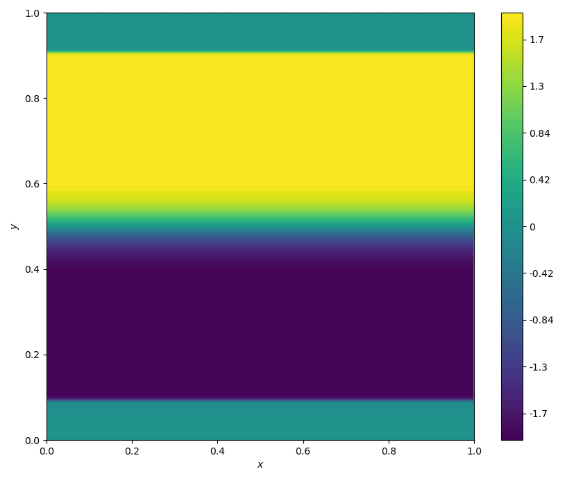
\includegraphics[width=\textwidth,height=0.85\textwidth]{Rusa2v.png}
		\caption{Vitesse suivant $y$}
		\label{fig:Rusa2v}
	\end{subfigure}
	\caption{Illustration de la résolution du système de Saint-Venant par le flux de Rusanov 2D. La condition initiale imposée est  $ h = 2$ pour $ 0.3 \leq y \leq 0.7$.}
	\label{fig:Rusa2}
\end{figure}


\begin{figure}[H]
	\centering
	\begin{subfigure}{0.32\textwidth}
		\centering
		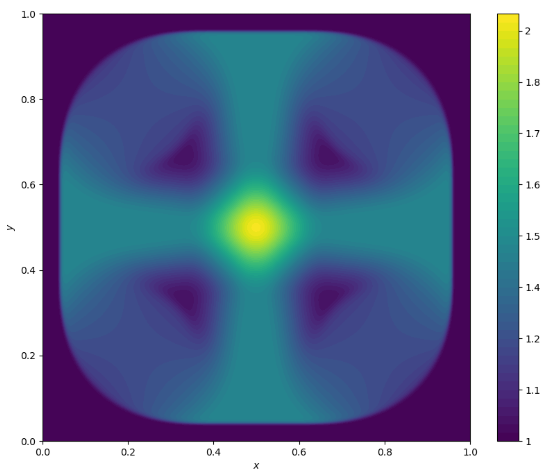
\includegraphics[width=\textwidth,height=0.85\textwidth]{Rusa3h.png}
		\caption{Hauteur d'eau}
		\label{fig:Rusa3h}
	\end{subfigure}
	\begin{subfigure}{0.32\textwidth}
		\centering
		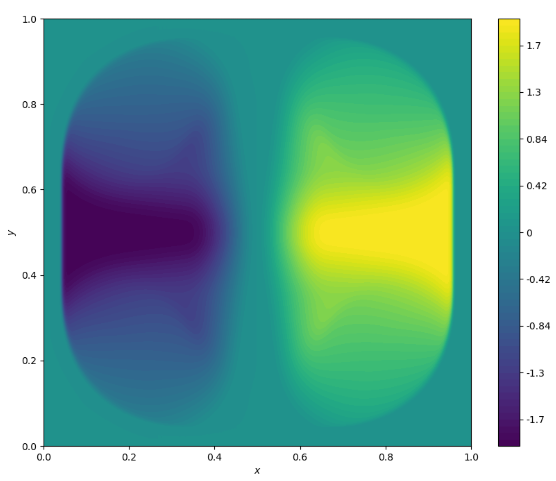
\includegraphics[width=\textwidth,height=0.85\textwidth]{Rusa3u.png}
		\caption{Vitesse suivant $x$}
		\label{fig:Rusa3u}
	\end{subfigure}
	\begin{subfigure}{0.32\textwidth}
		\centering
		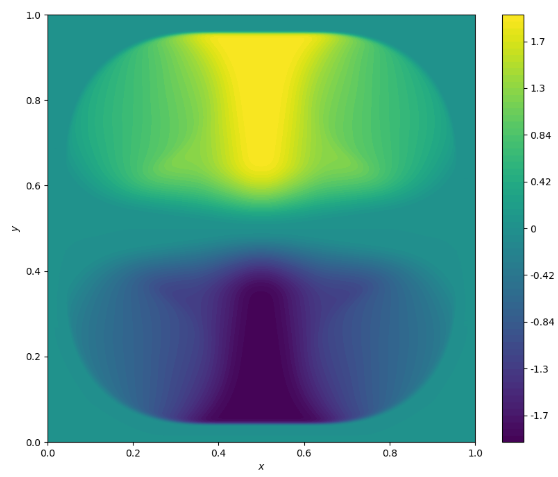
\includegraphics[width=\textwidth,height=0.85\textwidth]{Rusa3v.png}
		\caption{Vitesse suivant $y$}
		\label{fig:Rusa3v}
	\end{subfigure}
	\caption{Illustration de la résolution du système de Saint-Venant par le flux de Rusanov 2D. La condition initiale imposée est $ h = 2$ sur $[0.25,0.75]\times[0.25,0.75]$.}
	\label{fig:Rusa3}
\end{figure}

\noindent Ces figures nous montrent la propagation d'une onde de choc (une vague) vers les bords du domaine, et d'une onde de détente vers le centre du barrage. La \cref{fig:Rusa1h} permet d'observer la vidange complète de la zone de rétention d'eau (intérieur du barrage), et la \cref{fig:Rusa2h} capture le barrage en cours de la vidange \footnote{Remarquons que la forme du barrage est différente entre la \cref{fig:Rusa1} et la \cref{fig:Rusa2}}. Remarquons une vitesse suivant $y$ (resp. suivant $x$) nulle pour la \cref{fig:Rusa1v} (resp. pour la \cref{fig:Rusa2u}). La \cref{fig:Rusa3} permet d'illustrer une propagation des ondes simultanément dans les deux directions de l'espace. 

%----------------------------------------------------------------------
\subsection*{Question 4.}

\begin{problem}
	Description de l'utilisation du solveur de Riemann 1D pour l'adaptation aux calculs en 2D.
\end{problem}


\subsection*{Réponse} 

\textit{En 2D de façon générale, l'indice $L$ désigne l'état du centre et $R$ l'état voisin. Cependant, dans cette question, ils indiqueront les états de gauche, de droite, du bas, ou du haut du cellule en fonction de la direction du vecteur normal; ceci afin de faciliter les explications.}

Rappelons que dans le cas 1D, la valeur de $h^*$ (et par suite celle de $u^*$) aux interfaces, i.e. entre un état gauche $(h_L,u_L)$ et un état droit $(h_R,u_R)$ est donnée par la solution du problème suivant:
\begin{align*}
	u_L - (h^* - h_L)Z(h_L, h^*) = u_R + (h^* - h_R)Z(h_R, h^*)
\end{align*}
ou la fonction $Z(\cdot, \cdot)$ de classe $C^1$ est donnée par
\begin{align*}
	Z(a,b) = 
	\begin{cases}
		\frac{2\sqrt{g}}{\sqrt{a}+\sqrt{b}}	 &\qquad	\text{si} \quad b<a \\
		\sqrt{g}\sqrt{\frac{a+b}{2ab}}	 &\qquad	\text{si} \quad b>a 
	\end{cases}
\end{align*}
Cette équation résolue par la méthode de Newton permet de déterminer si on est présence d'une onde simple ou d'un choc; et le solveur de Riemann 1D permet enfin de calculer l'état du système $w = (h,u)$ en un point $x/t$ donné.

\noindent Pour adapter ce schéma en 2D, il suffit de remplacer la vitesse scalaire 1D $u$ par la composante normale $U \cdot n$, où $n=n_{LR} =(n_1, n_2)$, du vecteur vitesse 2D. Il faudra donc résoudre l'équation ci-bas en utilisant le solveur de Riemann 1D:
\begin{align*}
	U_L \cdot n - (h^* - h_L)Z(h_L, h^*) = U_R \cdot n + (h^* - h_R)Z(h_R, h^*)
\end{align*}
Une fois la composante normale du vecteur vitesse $U^* \cdot n$ à l'interface obtenue, il nous manque sa composante tangentielle $U^* \cdot n'$, où $n'= n'_{LR} = (-n_2, n_1)$. On peut la prendre égale à la composante tangentielle de l'état de gauche, ou de celui de droite, ou l'un des deux en fonction d'un critère pertinent. Autrement dit, 
\begin{align*}
	U^* \cdot n' = 
	\begin{cases}
		U_L \cdot n' &\qquad \text{si} \quad  U^* \cdot n > 0\\
		U_R \cdot n' &\qquad \text{sinon}
	\end{cases}
\end{align*}
Enfin, le vecteur vitesse à l'interface est obtenu en résolvant le système:
\begin{align*}
	U^* = 
	\begin{pmatrix} u^* \\ v^* \end{pmatrix}
	= (U^* \cdot n)n + (U^* \cdot n')n'
	= \begin{pmatrix} n_1 & -n_2 \\ n_2 & n_1 \end{pmatrix}
	\begin{pmatrix} U^* \cdot n \\ U^* \cdot n' \end{pmatrix}
\end{align*}



%----------------------------------------------------------------------
\subsection*{Question 5.}

\begin{problem}
	Description de l’implémentation des conditions aux limites suivantes: miroir, valeurs imposées, zone sèche.
\end{problem}

\subsection*{Réponse} 

\textit{Dans cette partie, l'indice $L$ désigne une cellule du bord du domaine, et l'indice $R$ une cellule fantôme se trouvant à l'extérieur du domaine. Afin de faciliter les écritures, désignons par $U^n$ et $U^t$ les composantes normales et tangentielles respectives.}

\subsubsection*{Zone miroir (cf. \cref{fig:Bord1})}
\begin{itemize}
	\item la hauteur d'eau à la limite est prise égale à celle de la cellule proche du bord: $h_R = h_L$
	\item la composante normale du vecteur vitesse est inversée: $U_R^n = -U_L^n$ 
	\item la composante tangentielle du vecteur vitesse est maintenue: $U_R^t = U_L^t$
\end{itemize}
Au final, le vecteur vitesse sur le bord donne
\begin{align*}
	U_R &= -U^n_L + U^t_L \\
	&= -U^n_L + (U_L -U^n_L) \\
	&= U_L - 2(U_L \cdot n)n 
\end{align*}  

\subsubsection*{Valeurs imposées (cf. \cref{fig:Bord2})}
\begin{itemize}
	\item la hauteur d'eau $h_R$ est donnée
	\item les composantes normales $U_R^n$ et tangentielles $U_R^t$ du vecteur vitesse sont données 
\end{itemize}
Si seulement le module du vecteur vitesse $\Vert U_R \Vert_2$ est donnée sur le bord, on pourra prendre $U_R^n = \Vert U_R \Vert_2 n$, et prendre $U_R^t = (0,0)$.

\subsubsection*{Zone sèche (cf. \cref{fig:Bord3})}
\begin{itemize}
	\item la hauteur d'eau $h_R = 0$ par définition. Cependant cette condition est difficile à implémenter. On prendra donc une hauteur suffisamment faible, par exemple $h_R = 0.05$.
	\item pour $h_R=0$, la vitesse n'est pas définie. On peut prendre $U_R = (0,0)$ si on impose $h_R = 0.05$.
\end{itemize}

\subsubsection*{Illustrations}
Observons à présents quelques résultats en appliquant ces conditions aux limites. La condition initiale est celle d'une rupture d'un barrage en forme de carré: $h = 2$ sur $[0.25,0.75]\times[0.25,0.75]$ et $h=1$ ailleurs. Le temps final est $t_{max} = 0.7$ afin que les vagues atteignent les bords du domaine. Les problèmes sont résolus en utilisant le flux de Rusanov 2D.

\begin{figure}[H]
	\centering
	\begin{subfigure}{0.32\textwidth}
		\centering
		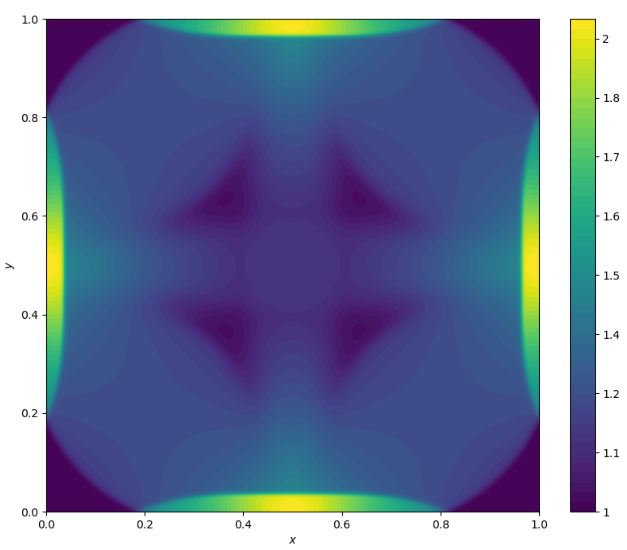
\includegraphics[width=\textwidth,height=0.85\textwidth]{Bord1h.png}
		\caption{Hauteur d'eau}
		\label{fig:Bord1h}
	\end{subfigure}
	\begin{subfigure}{0.32\textwidth}
		\centering
		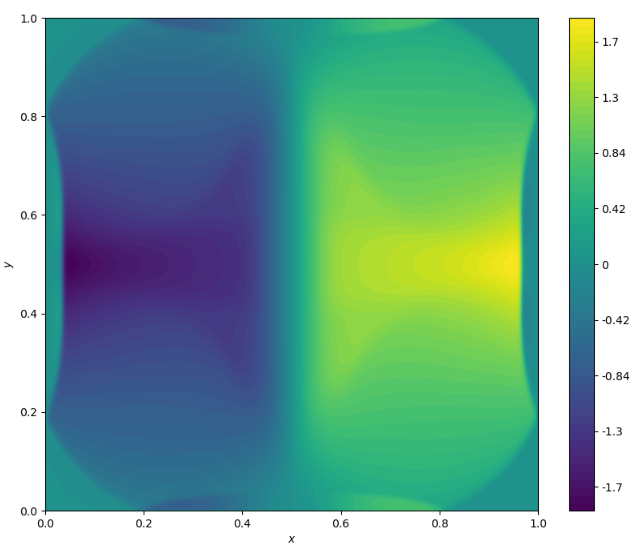
\includegraphics[width=\textwidth,height=0.85\textwidth]{Bord1u.png}
		\caption{Vitesse suivant $x$}
		\label{fig:Bord1u}
	\end{subfigure}
	\begin{subfigure}{0.32\textwidth}
		\centering
		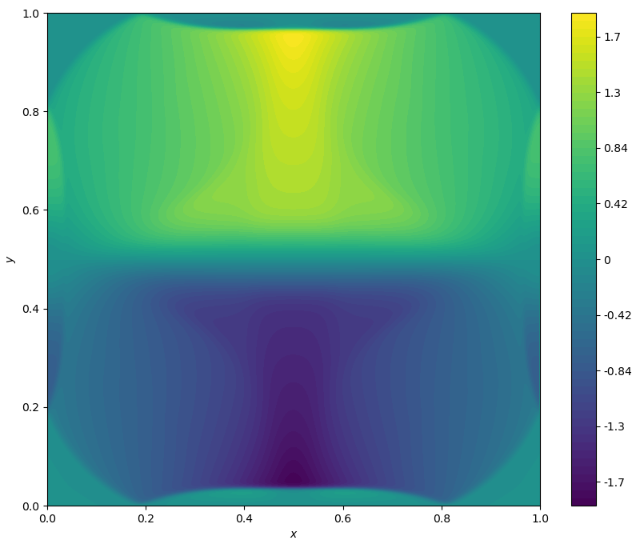
\includegraphics[width=\textwidth,height=0.85\textwidth]{Bord1v.png}
		\caption{Vitesse suivant $y$}
		\label{fig:Bord1v}
	\end{subfigure}
	\caption{Illustration des conditions aux limites de type miroir. Ce cas peu être assimilé à un bassin (ou une piscine, etc.) ayant des propriétés réflectives sur ses bords.}
	\label{fig:Bord1}
\end{figure}


\begin{figure}[H]
	\centering
	\begin{subfigure}{0.32\textwidth}
		\centering
		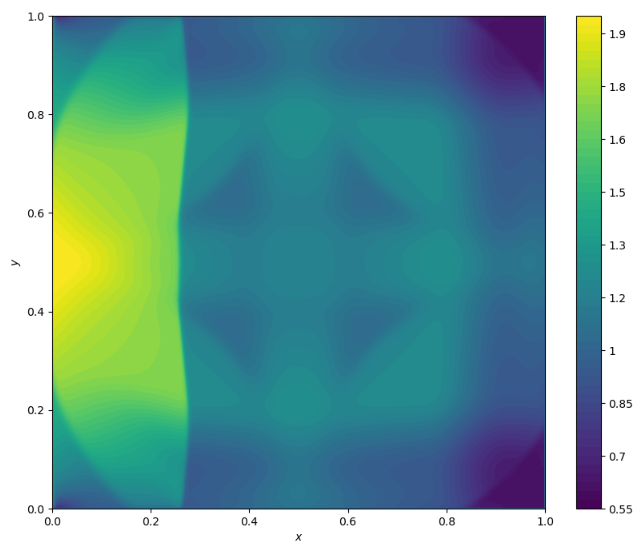
\includegraphics[width=\textwidth,height=0.85\textwidth]{Bord2h.png}
		\caption{Hauteur d'eau}
		\label{fig:Bord2h}
	\end{subfigure}
	\begin{subfigure}{0.32\textwidth}
		\centering
		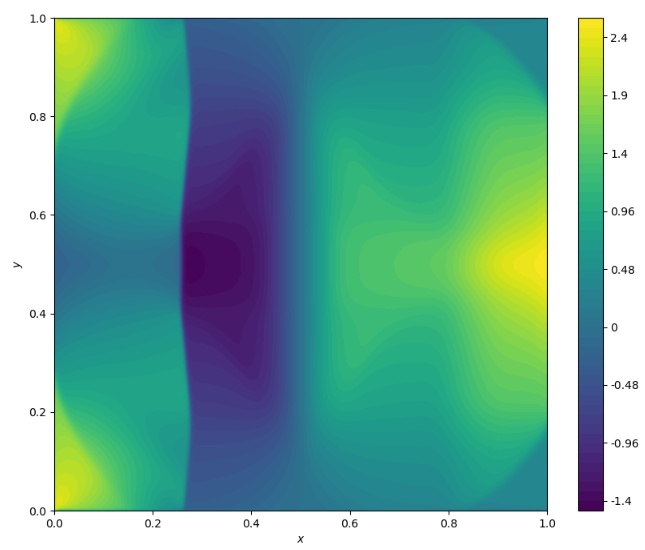
\includegraphics[width=\textwidth,height=0.85\textwidth]{Bord2u.png}
		\caption{Vitesse suivant $x$}
		\label{fig:Bord2u}
	\end{subfigure}
	\begin{subfigure}{0.32\textwidth}
		\centering
		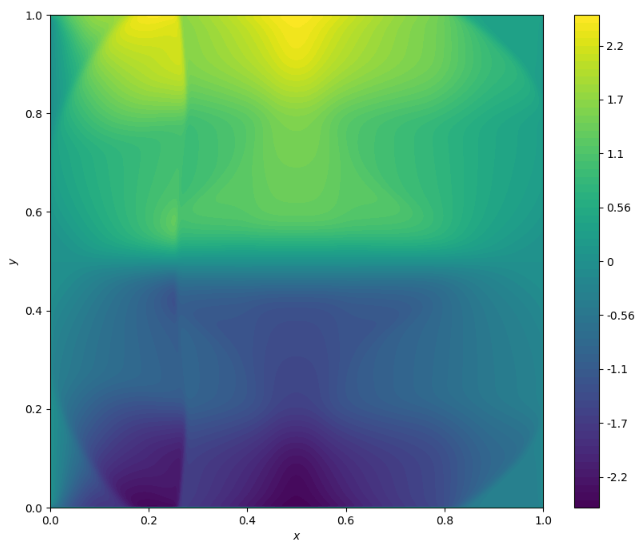
\includegraphics[width=\textwidth,height=0.85\textwidth]{Bord2v.png}
		\caption{Vitesse suivant $y$}
		\label{fig:Bord2v}
	\end{subfigure}
	\caption{Illustration des conditions aux limites de type valeurs imposées. Ce cas peut être assimilé à un bassin contenant un barrage situé sur le lit d'un fleuve. En amont (sur la gauche), on applique la condition $h_R=1.5$, $(u_R,v_R)=(1.5,0)$; en aval (et sur les deux autres bords), on applique $h_R=0.5$, $(u_R,v_R)=(0,0)$. On observe que le barrage est vite rempli et le fleuve continue son écoulement.}
	\label{fig:Bord2}
\end{figure}


\begin{figure}[H]
	\centering
	\begin{subfigure}{0.32\textwidth}
		\centering
		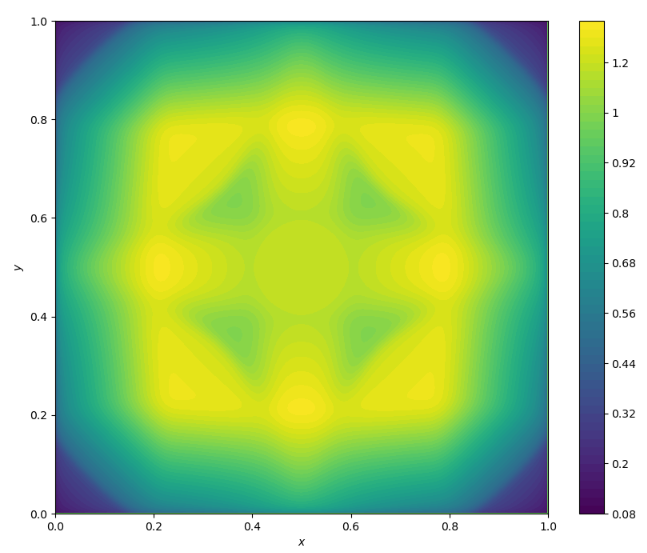
\includegraphics[width=\textwidth,height=0.85\textwidth]{Bord3h.png}
		\caption{Hauteur d'eau}
		\label{fig:Bord3h}
	\end{subfigure}
	\begin{subfigure}{0.32\textwidth}
		\centering
		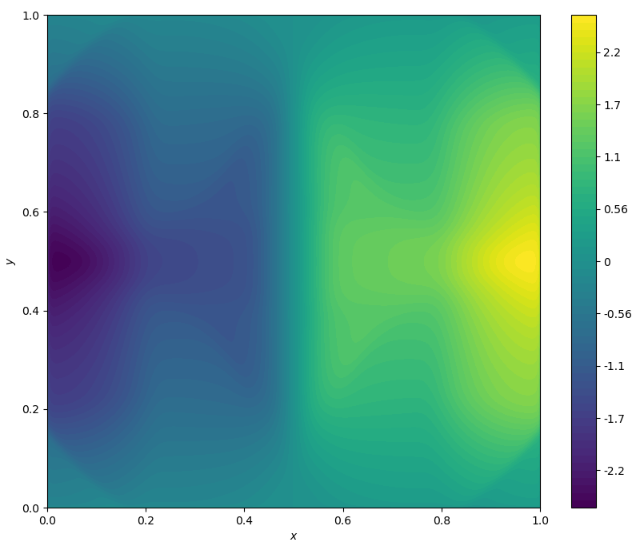
\includegraphics[width=\textwidth,height=0.85\textwidth]{Bord3u.png}
		\caption{Vitesse suivant $x$}
		\label{fig:Bord3u}
	\end{subfigure}
	\begin{subfigure}{0.32\textwidth}
		\centering
		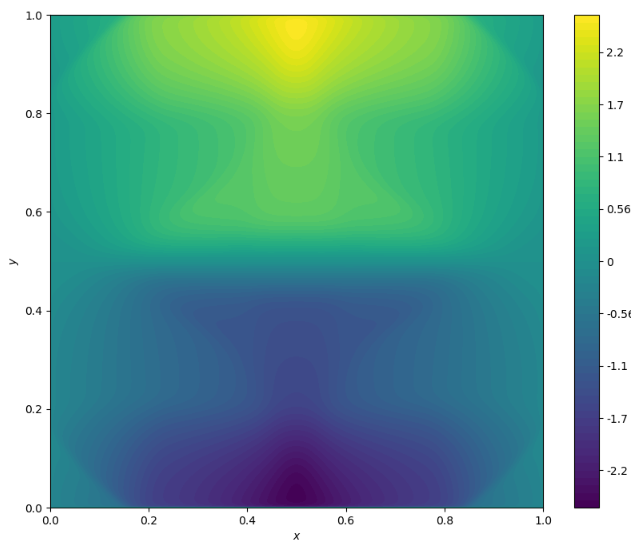
\includegraphics[width=\textwidth,height=0.85\textwidth]{Bord3v.png}
		\caption{Vitesse suivant $y$}
		\label{fig:Bord3v}
	\end{subfigure}
	\caption{Illustration des conditions aux limites de type zone sèche. On prend $h_R$ presque nul sur les bords du domaine, et une vitesse nulle i.e $h_R=0.05$, $(u_R,v_R)=(0,0)$.}
	\label{fig:Bord3}
\end{figure}


%----------------------------------------------------------------------
\subsection*{Question 6.}

\begin{problem}
	Mise en oeuvre de la résolution du système de Saint-Venant sur un maillage volume fini régulier. Vérifions la validité de la programmation en calculant d'abord des solutions de problème de Riemann dans la direction $x$ puis dans la direction $y$ avec un fond plat $(A = cste)$.
\end{problem}

\subsection*{Réponse} 

Les modifications de test demandées ont été préalablement effectuées et implémentées aux \cref{fig:Rusa1,fig:Rusa2} pour tester notre implémentation du flux de Rusanov 2D. À présent, reprenons les mêmes paramètres (ceux indiqués à la question 3.) pour vérifier notre programmation du solveur de Riemann 2D. Les fonds utilisés seront plats, et à l'altitude nulle i.e $A(\cdot,\cdot) \equiv 0$


\begin{figure}[H]
	\centering
	\begin{subfigure}{0.32\textwidth}
		\centering
		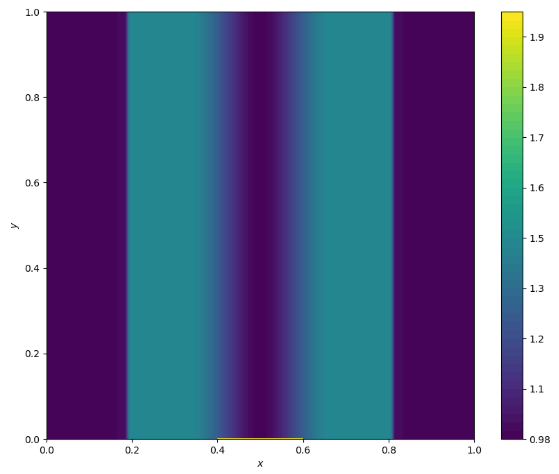
\includegraphics[width=\textwidth,height=0.85\textwidth]{Riem1h.png}
		\caption{Hauteur d'eau}
		\label{fig:Riem1h}
	\end{subfigure}
	\begin{subfigure}{0.32\textwidth}
		\centering
		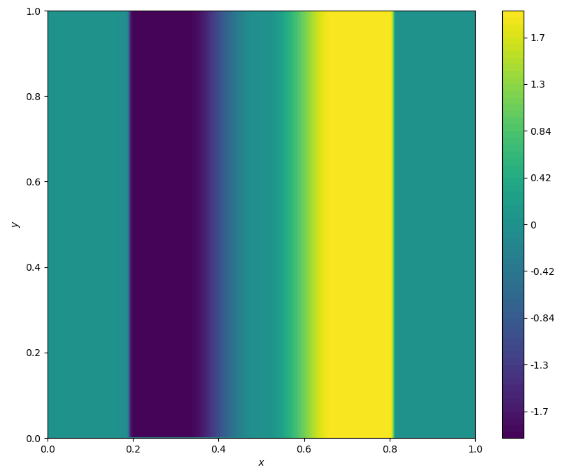
\includegraphics[width=\textwidth,height=0.85\textwidth]{Riem1u.png}
		\caption{Vitesse suivant $x$}
		\label{fig:Riem1u}
	\end{subfigure}
	\begin{subfigure}{0.32\textwidth}
		\centering
		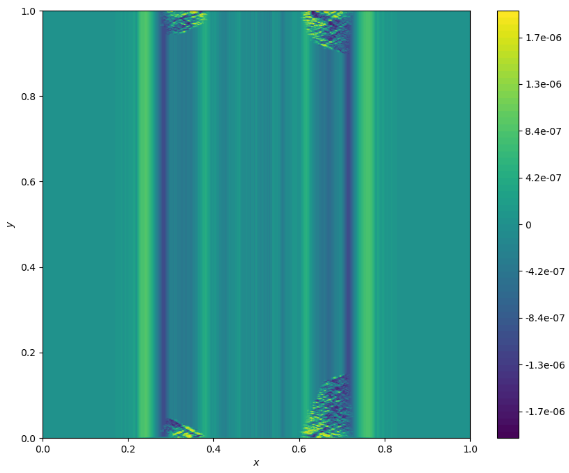
\includegraphics[width=\textwidth,height=0.85\textwidth]{Riem1v.png}
		\caption{Vitesse suivant $y$}
		\label{fig:Riem1v}
	\end{subfigure}
	\caption{Illustration de la résolution du système de Saint-Venant par le solveur de Riemann 2D. La condition initiale imposée est  $ h = 2$ pour $ 0.4 \leq x \leq 0.6$, afin d'obtenir un calcul des solutions du problème de Riemann dans la direction $x$.}
	\label{fig:Riem1}
\end{figure}

\begin{figure}[H]
	\centering
	\begin{subfigure}{0.32\textwidth}
		\centering
		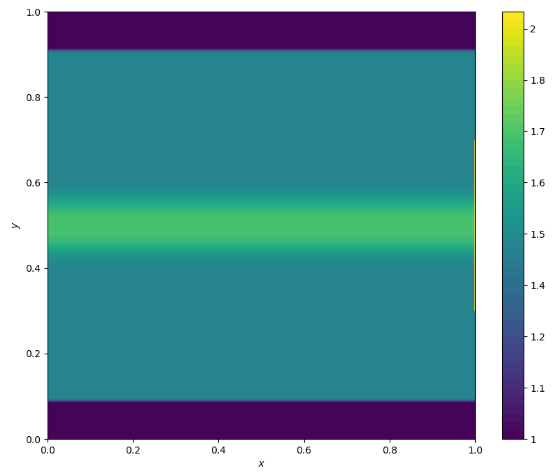
\includegraphics[width=\textwidth,height=0.85\textwidth]{Riem2h.png}
		\caption{Hauteur d'eau}
		\label{fig:Riem2h}
	\end{subfigure}
	\begin{subfigure}{0.32\textwidth}
		\centering
		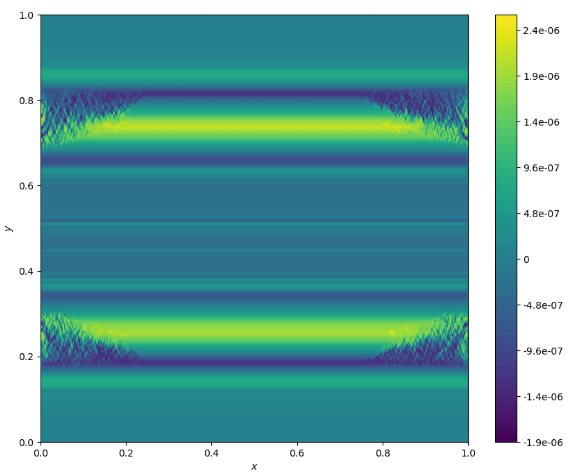
\includegraphics[width=\textwidth,height=0.85\textwidth]{Riem2u.png}
		\caption{Vitesse suivant $x$}
		\label{fig:Riem2u}
	\end{subfigure}
	\begin{subfigure}{0.32\textwidth}
		\centering
		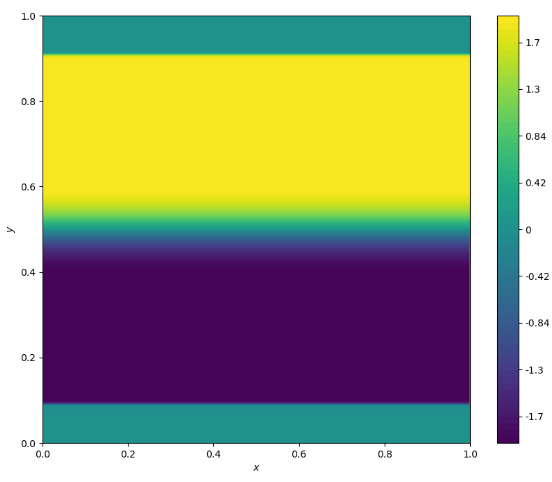
\includegraphics[width=\textwidth,height=0.85\textwidth]{Riem2v.png}
		\caption{Vitesse suivant $y$}
		\label{fig:Riem2v}
	\end{subfigure}
	\caption{Illustration de la résolution du système de Saint-Venant par le solveur de Riemann 2D. La condition initiale imposée est $ h = 2$ pour $ 0.3 \leq y \leq 0.7$, afin d'obtenir un calcul des solutions du problème de Riemann dans la direction $y$.}
	\label{fig:Riem2}
\end{figure}

\noindent On observe aux \cref{fig:Riem1u,fig:Riem2v} qu'effectivement, le calcul de solutions du problème de Riemann se fait dans la direction normale de propagation de l'onde (i.e $x$ pour la \cref{fig:Riem1u} et $y$ pour la \cref{fig:Riem2v}). Tout ceci implique des vitesses tangentielles nulles, ce que nous observons aux \cref{fig:Riem1v,fig:Riem2u}.


%----------------------------------------------------------------------
\subsection*{Question 7.}

\begin{problem}
	Testons notre programme sur un cas 2D avec un fond plat.
\end{problem}

\subsection*{Réponse} 
Comme pour les cas précédents, le fond utilisés sera plat à l'altitude nulle i.e $A(\cdot,\cdot) \equiv 0$. 


\begin{figure}[H]
	\centering
	\begin{subfigure}{0.32\textwidth}
		\centering
		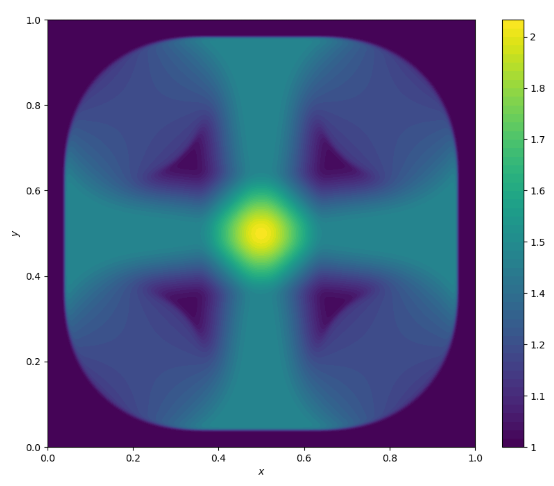
\includegraphics[width=\textwidth,height=0.85\textwidth]{Riem3h.png}
		\caption{Hauteur d'eau}
		\label{fig:Riem3h}
	\end{subfigure}
	\begin{subfigure}{0.32\textwidth}
		\centering
		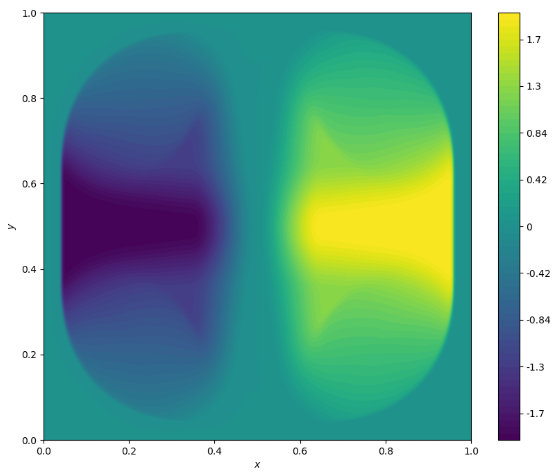
\includegraphics[width=\textwidth,height=0.85\textwidth]{Riem3u.png}
		\caption{Vitesse suivant $x$}
		\label{fig:Riem3u}
	\end{subfigure}
	\begin{subfigure}{0.32\textwidth}
		\centering
		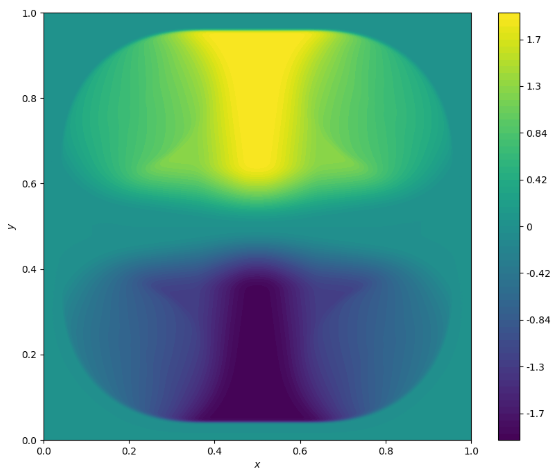
\includegraphics[width=\textwidth,height=0.85\textwidth]{Riem3v.png}
		\caption{Vitesse suivant $y$}
		\label{fig:Riem3v}
	\end{subfigure}
	\caption{Illustration de la résolution du système de Saint-Venant par le solveur de Riemann 2D. La condition initiale imposée est $ h = 2$ sur $[0.25,0.75]\times[0.25,0.75]$. Cette figure correspond au même cas test que nous avons utilisé pour le flux de Rusanov 2D (cf. \cref{fig:Rusa3}); il permet d'observer l'exactitude des résultats.}
	\label{fig:Riem3}
\end{figure}


\begin{figure}[H]
	\centering
	\begin{subfigure}{0.32\textwidth}
		\centering
		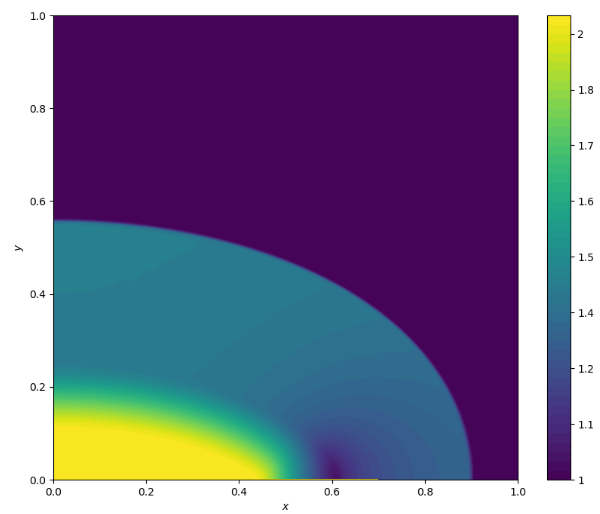
\includegraphics[width=\textwidth,height=0.85\textwidth]{Riem4h.png}
		\caption{Hauteur d'eau}
		\label{fig:Riem4h}
	\end{subfigure}
	\begin{subfigure}{0.32\textwidth}
		\centering
		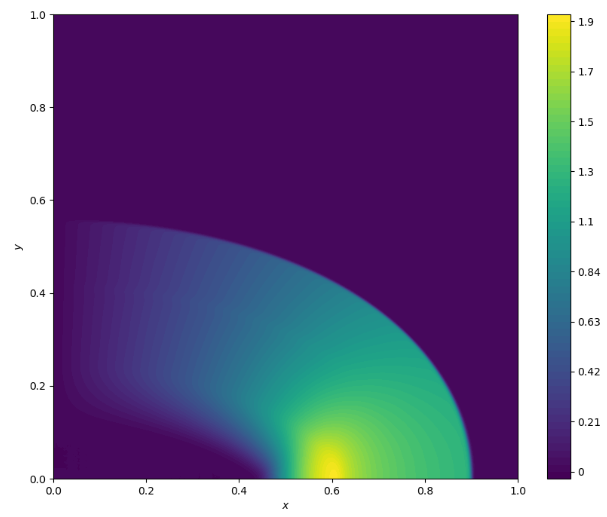
\includegraphics[width=\textwidth,height=0.85\textwidth]{Riem4u.png}
		\caption{Vitesse suivant $x$}
		\label{fig:Riem4u}
	\end{subfigure}
	\begin{subfigure}{0.32\textwidth}
		\centering
		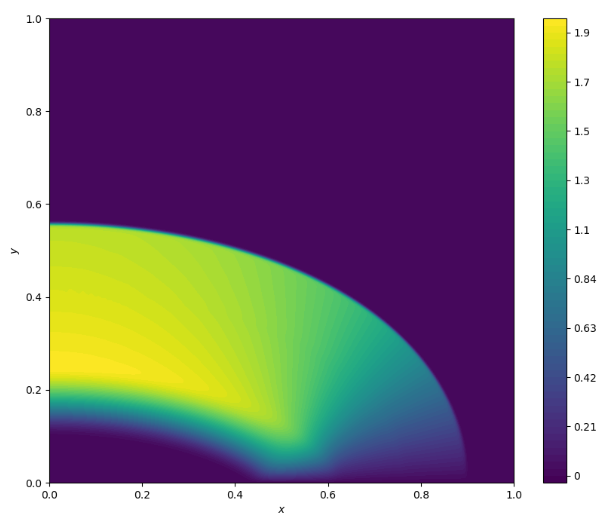
\includegraphics[width=\textwidth,height=0.85\textwidth]{Riem4v.png}
		\caption{Vitesse suivant $y$}
		\label{fig:Riem4v}
	\end{subfigure}
	\caption{Illustration de la résolution du système de Saint-Venant par le solveur de Riemann 2D sur un cas non-symétrique. La condition initiale imposée est $h = 2$ à l intérieur de quadrant d'ellipse $\sfrac{x^2}{4} + y^2 \leq 0.35^2$. Les conditions de bord qui sont appliquées sont celles de zones miroirs. Ce cas permet d'observer une dépression qui se forme autour de l'ellipse.}
	\label{fig:Riem4}
\end{figure}


%----------------------------------------------------------------------
\subsection*{Question 8.}

\begin{problem}
	Description et programmation la méthode MUSCL en 2D. 
\end{problem}

\subsection*{Réponse} 
Commençons par rappeler que le schéma de volumes finis en 2D s'écrit à l'itération $n$ comme suit 
\begin{align}
	\label{eq:num2d}
	w^{n+1}_L = w^n_L + \frac{\Delta t}{\vert L \vert } \sum_{R\in V(L)} \vert L/R \vert f(w^n_L, w^n_R, n_{LR})
\end{align}
où
\begin{itemize}
	\item $L$ désigne les carrés (ou mailles, ou volumes finis) de quadratures
	\item $V(L)$ l'ensemble des voisins $R$ de $L$
	\item $\vert L \vert$ la surface de $L$
	\item $\vert L/R \vert$ longueur de l'interface entre $L$ et $R$
	\item la fonction $f$ désigne le flux numérique\footnote{Il s'agira dans cas du flux de Rusanov dont on voudrait améliorer la précision}
\end{itemize}

L'idée de la méthode MUSCL est de remplacer le flux numérique calculé aux points $w^n_L$ et $w^n_R$ par un flux numérique calculé en des points plus proches de l'interfaces, et à un pas de temps correspondant. On notera ces points par $w^*_L$ et $w^*_R$. On pose alors


\begin{equation}	
	\label{eq:muscl}
	\begin{aligned}
		w^*_L &= w^n_L +  \frac{\Delta x}{2} s_{x_L} + \frac{\Delta y}{2} s_{y_L} + \frac{\Delta t}{2} r^n_{L} \\
		w^*_R &= w^n_R - \frac{\Delta x}{2} s_{x_R} - \frac{\Delta y}{2} s_{y_R} + \frac{\Delta t}{2} r^n_{R}
	\end{aligned}
\end{equation}

Pour le calcul des pentes en espace $s^n_{x_L}$ et $s^n_{y_L}$ pour une maille quelconque $L$, on distingue 4 possibilités pour les cellules du bord:
\begin{itemize}
	\item $w_{right}$ correspondant au voisin de droite 
	\item $w_{left}$ correspondant au voisin de gauche
	\item $w_{up}$ correspondant au voisin du haut
	\item $w_{down}$ correspondant au voisin bas 
\end{itemize}
On pose ensuite
\begin{align*}
	\alpha_x = \frac{w^n_L - w^n_{left}}{\Delta x}, \quad
	\beta _x = \frac{w^n_{right} - w^n_{L}}{\Delta x}, \quad
	\gamma _x = \frac{w^n_{right} - w^n_{left}}{2\Delta x}
\end{align*}
De façon similaire, on pose
\begin{align*}
	\alpha_y = \frac{w^n_L - w^n_{down}}{\Delta y}, \quad
	\beta _y = \frac{w^n_{up} - w^n_{L}}{\Delta y}, \quad
	\gamma _y = \frac{w^n_{up} - w^n_{down}}{2\Delta y}
\end{align*}
On en déduit les pentes en espace
\begin{align*}
	s^n_{x_L} = \text{minmod}(\alpha_x, \beta _x, \gamma _x) \\
	s^n_{y_L} = \text{minmod}(\alpha_y, \beta _y, \gamma _y)
\end{align*}
où la fonction $\text{minmod}$\footnote{Notons que ces quantités sont des vecteurs, et donc la fonction $\text{minmod}$ doit être appliquée composante par composante} est donnée par:
\begin{align*}
	\text{minmod}(\alpha, \beta, \gamma) = 
	\begin{cases}
		\min(\alpha, \beta, \gamma) \qquad &\text{si  } \alpha,\beta,\gamma > 0 \\
		\max(\alpha, \beta, \gamma) \qquad &\text{si  } \alpha,\beta,\gamma < 0 \\
		0 \qquad &\text{sinon  }
	\end{cases}
\end{align*}

Pour le calcul des pentes en temps, on se sert des matrices jacobiennes des composants du flux physique $f_1$ et $f_2$. D'après $(\mathcal{S}')$, on a
$$
\partial_t w + \partial_x f_1(w) + \partial_y f_2(w) = S(w)
$$
On prend donc la pente $r^n_L$ telle que 
$$
r^n_L = - \frac{\partial f_1}{\partial w} (w^n_L) s_{x_L} - \frac{\partial f_2}{\partial w} (w^n_L) s_{y_L} + S(w) 
$$ 


Les pentes $s^n_{x_L}$, $s^n_{y_L}$ et  $r^n_L$ ayant été calculées, on calcule le flux numérique aux points $w^*_L$ et $w^*_R$ grâce à l'\cref{eq:muscl}, qu'on applique au schéma numérique. L'\cref{eq:num2d} devient alors
\begin{align}
	w^{n+1}_L = w^n_L + \frac{\Delta t}{\vert L \vert } \sum_{R\in V(L)} \vert L/R \vert f(w^*_L, w^*_R, n_{LR})
\end{align}

En pratique, les pentes sont calculées indépendamment des états $w$, dans leur kernel propres. 
Le code de calcul est donné ci bas \footnote{Les fonctions de calcul $\text{minmod}$ et celles des matrices jacobiennes de $f_1$ et $f_2$, triviales, ne sont pas décrites dans ce rapport.}. Les pentes $s^n_{x_L}$, $s^n_{y_L}$ et $r^n_L$ y sont repérées respectivement par $\verb|dxwn|$, $\verb|dywn|$, et $\verb|dtwn|$.


\begin{lstlisting}[language=C, caption={Kernel de calcul des pentes en espace et en temps pour la méthode MUSCL},breaklines]
__kernel void muscl(__global const float *wn, __global float *dxwn, __global float *dywn, __global float *dtwn){
	int id = get_global_id(0);
	int i = id % _NX;
	int j = id / _NX;
	int ngrid = _NX * _NY;
	// Juste les cellules internes
	if (i > 0 && i < _NX - 1 && j > 0 && j < _NY - 1){
	double w[_M];
	for(int iv = 0; iv < _M; iv++){
		int imem = i + j * _NX + iv * ngrid;
		w[iv] = wn[imem];
	}
	double wR[_M];
	double wL[_M];
	double wU[_M];
	double wD[_M];
	for(int idir = 0; idir < 4; idir++){
		int iR = i + dir[idir][0];
		int jR = j + dir[idir][1];
		for(int iv = 0; iv < _M; iv++){ 
			int imem = iv * ngrid + iR + jR * _NX;
			if (idir == 0)
				wR[iv] = wn[imem];
			else if (idir == 1)
				wL[iv] = wn[imem];
			else if (idir == 2)
				wU[iv] = wn[imem];
			else if (idir == 3)
				wD[iv] = wn[imem];
		}
	}
	// Calcul des pentes en espace
	float dxLoc[_M];
	float dyLoc[_M];
	for(int iv = 0; iv < _M; iv++){ 
		int imem = i + j * _NX + iv * ngrid;
		// Cacul de dxwn
		double alpha = (w[iv] - wL[iv]) / _DX;
		double beta = (wR[iv] - w[iv]) / _DX;
		double gamma = (wR[iv] - wL[iv]) / (2*_DX);
		dxLoc[iv] = minmod(alpha, beta, gamma);
		dxwn[imem] = dxLoc[iv];

		// Cacul de dywn
		alpha = (w[iv] - wD[iv]) / _DY;
		beta = (wU[iv] - w[iv]) / _DY;
		gamma = (wU[iv] - wD[iv]) / (2*_DY);
		dyLoc[iv] = minmod(alpha, beta, gamma);
		dywn[imem] = dyLoc[iv];
	}
	// Cacul des pentes en temps
	double f1Prime[9]; 
	double f2Prime[9]; 
	fluxPrime(w, f1Prime, f2Prime);
	float dtLoc[3];
		for (int iLoc = 0; iLoc < 3; iLoc++){
			int imem = i + j * _NX + iLoc * ngrid;

			dtLoc[iLoc] = 0;
			for (int jLoc = 0; jLoc < 3; jLoc++){
				int index = iLoc*3 + jLoc;
				dtLoc[iLoc] -= (f1Prime[index]*dxLoc[jLoc] + f2Prime[index]*dyLoc[jLoc]);
			}

			dtwn[imem] = dtLoc[iLoc];
		}
	}
	// Pour gerer les pentes du bords
	else {
		for (int iv =0 ; iv < 3; iv++){
			int imem = i + j * _NX + iv * ngrid;
			dxwn[imem] = 0; 
			dywn[imem] = 0; 
			dtwn[imem] = 0; 
		}
	}
}
\end{lstlisting}
Les pentes ayant été calculées en amont, l'autre étape cruciale de l'implémentation de la méthode MUSCL est l'application des pentes $s^n_{x_L}$, $s^n_{y_L}$ et $r^n_L$ susmentionnée. Elles sont repérées dans le code ci-bas respectivement par $\verb|six|$, $\verb|siy|$, et $\verb|ri|$.

\begin{lstlisting}[language=C, caption={Application de la méthode MSUCL au flux de Rusanov},breaklines]
// Application des pentes en wL et wR 
// vn désigne le vecteur normal orienté de L vers R
for(int iv = 0; iv < _M; iv++){
	// wnow indique l'état actuel de la cellule
	wL[iv] = wnow[iv] + vn[0]*six[iv]*(_DX/2.0) + vn[1]*siy[iv]*(_DY/2.0) + ri[iv]*(_DT/2.0);

	// wR indique l'état de la cellule R
	wR[iv] = wR[iv] - vn[0]*sixR[iv]*(_DX/2.0) - vn[1]*siyR[iv]*(_DY/2.0) + riR[iv]*(_DT/2.0);
}  

// Application de MUSCL au flux de Rusanov 2D
flux_rusa_2d(wL, wR, vn, flux);                      
\end{lstlisting}

Nous testons la méthode sur deux cas étudiés aux questions précédentes.

\begin{figure}[H]
	\centering
	\begin{subfigure}{0.32\textwidth}
		\centering
		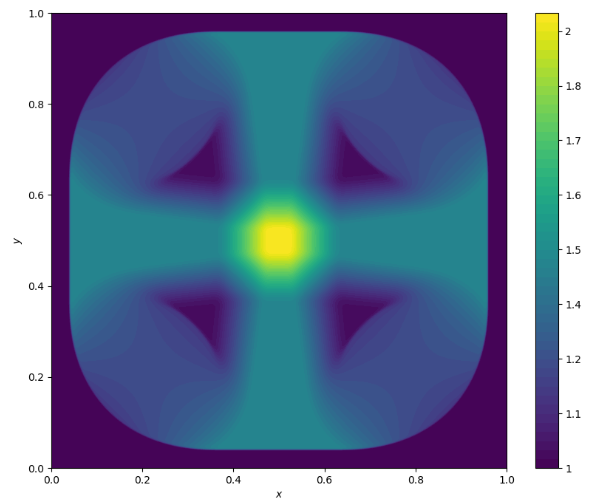
\includegraphics[width=\textwidth,height=0.85\textwidth]{Muscl1h.png}
		\caption{Hauteur d'eau}
		\label{fig:Muscl1h}
	\end{subfigure}
	\begin{subfigure}{0.32\textwidth}
		\centering
		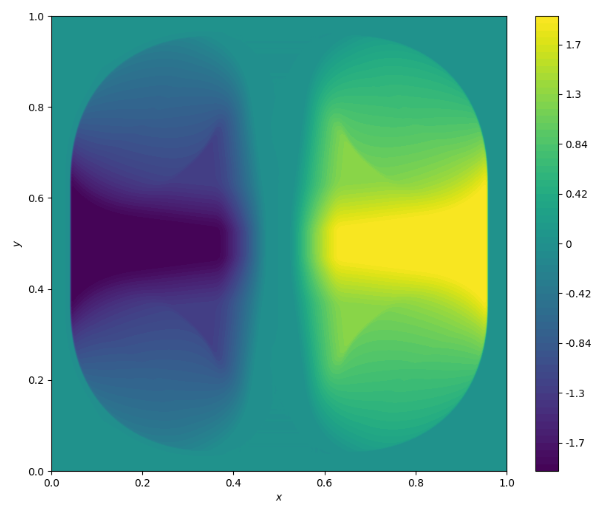
\includegraphics[width=\textwidth,height=0.85\textwidth]{Muscl1u.png}
		\caption{Vitesse suivant $x$}
		\label{fig:Muscl1u}
	\end{subfigure}
	\begin{subfigure}{0.32\textwidth}
		\centering
		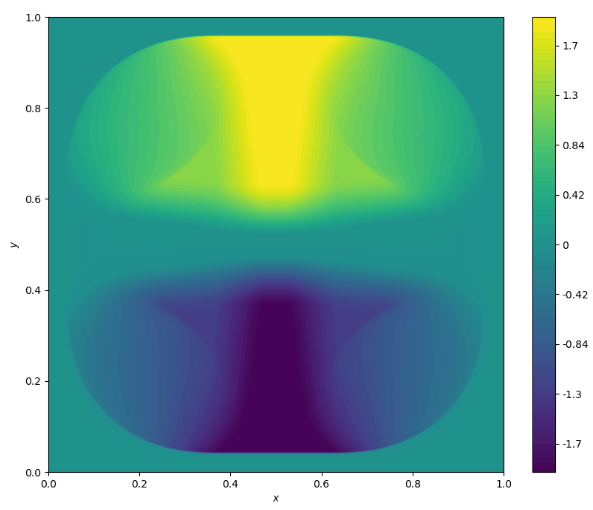
\includegraphics[width=\textwidth,height=0.85\textwidth]{Muscl1v.png}
		\caption{Vitesse suivant $y$}
		\label{fig:Muscl1v}
	\end{subfigure}
	\caption{Illustration de la résolution du système de Saint-Venant par la correction MUSCL appliquée au flux de Rusanov 2D. Comparé à la \cref{fig:Rusa3}, et en observant de près les hauteurs d'eau, on observe une nette amélioration.}
	\label{fig:Muscl1}
\end{figure}


\begin{figure}[H]
	\centering
	\begin{subfigure}{0.32\textwidth}
		\centering
		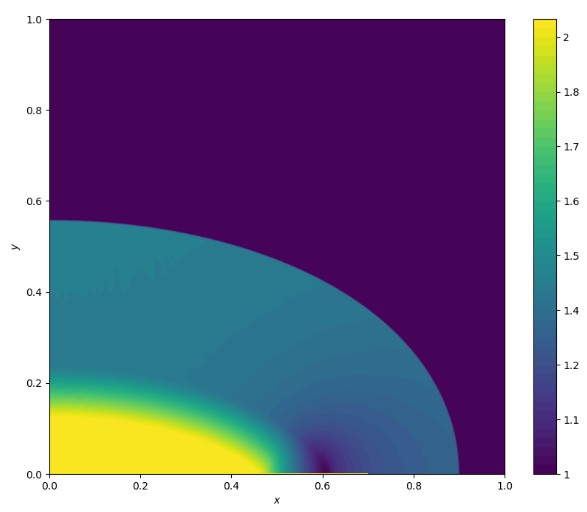
\includegraphics[width=\textwidth,height=0.85\textwidth]{Muscl2h.png}
		\caption{Hauteur d'eau}
		\label{fig:Muscl2h}
	\end{subfigure}
	\begin{subfigure}{0.32\textwidth}
		\centering
		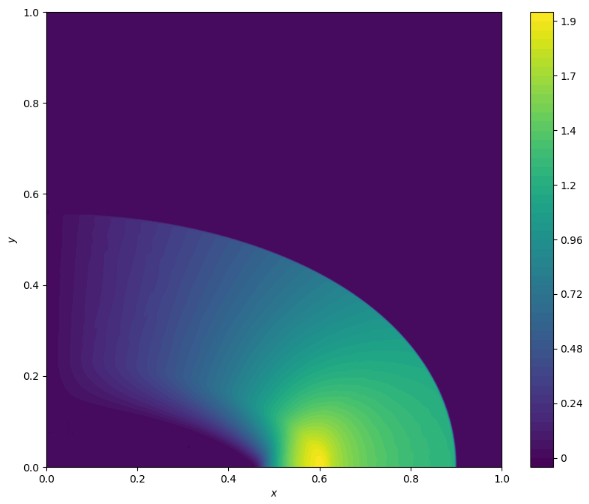
\includegraphics[width=\textwidth,height=0.85\textwidth]{Muscl2u.png}
		\caption{Vitesse suivant $x$}
		\label{fig:Muscl2u}
	\end{subfigure}
	\begin{subfigure}{0.32\textwidth}
		\centering
		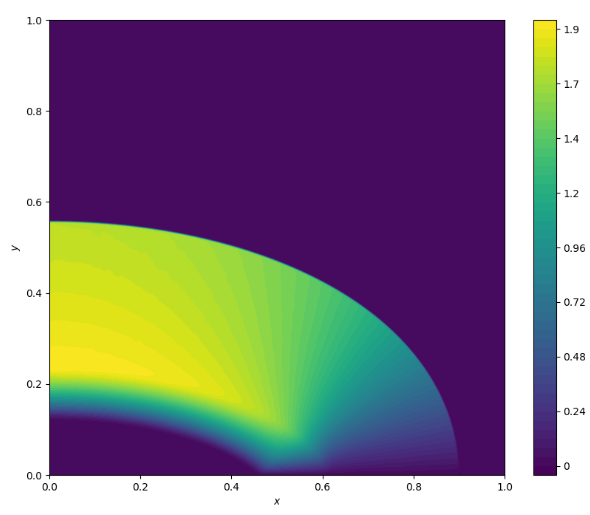
\includegraphics[width=\textwidth,height=0.85\textwidth]{Muscl2v.png}
		\caption{Vitesse suivant $y$}
		\label{fig:Muscl2v}
	\end{subfigure}
	\caption{Illustration de la résolution du système de Saint-Venant par la correction MUSCL appliquée au flux de Rusanov 2D sur un cas non-symétrique. Les conditions appliquées sont celles de la \cref{fig:Riem4}; en particulier la condition aux limites qui correspond à une zone miroir.}
	\label{fig:Muscl2}
\end{figure}


\begin{figure}[H]
	\centering
	\begin{subfigure}{0.32\textwidth}
		\centering
		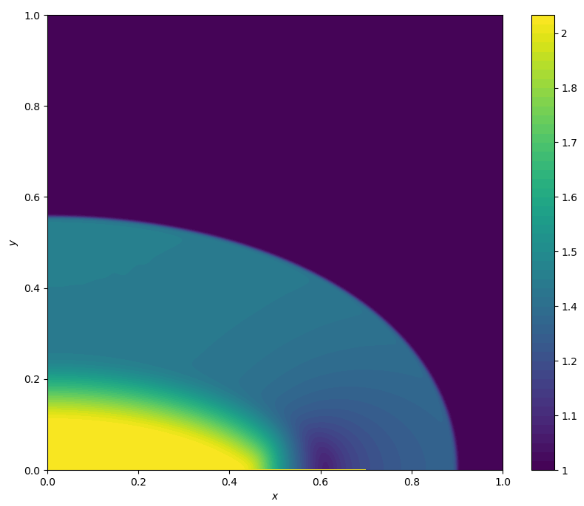
\includegraphics[width=\textwidth,height=0.85\textwidth]{Rusa4h.png}
		\caption{Hauteur d'eau}
		\label{fig:Rusa4h}
	\end{subfigure}
	\begin{subfigure}{0.32\textwidth}
		\centering
		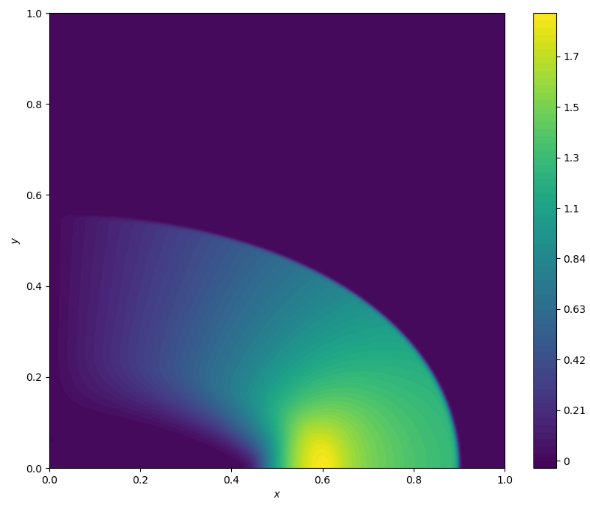
\includegraphics[width=\textwidth,height=0.85\textwidth]{Rusa4u.png}
		\caption{Vitesse suivant $x$}
		\label{fig:Rusa4u}
	\end{subfigure}
	\begin{subfigure}{0.32\textwidth}
		\centering
		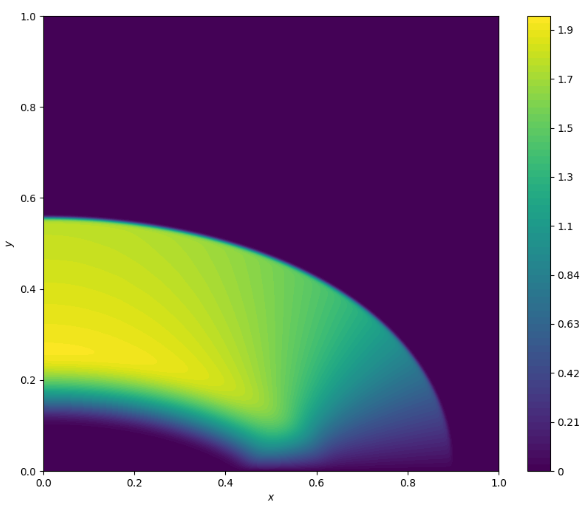
\includegraphics[width=\textwidth,height=0.85\textwidth]{Rusa4v.png}
		\caption{Vitesse suivant $y$}
		\label{fig:Rusa4v}
	\end{subfigure}
	\caption{Illustration de la résolution du système de Saint-Venant par le flux de Rusanov 2D sans correction MUSCL. Une fois de plus, comparé à la \cref{fig:Muscl2}, on observe une nette perte de précision, en particulier au niveau de la zone entourant le barrage.}
	\label{fig:Rusa4}
\end{figure}


%----------------------------------------------------------------------
\subsection*{Question 9.}

\begin{problem}
	Description des modifications à apporter au code pour traiter un fond quelconque.
\end{problem}

\subsection*{Réponse} 
Le flux considéré est un ajustement du flux de Rusanov $f$, noté $g$. On pose
\begin{align*}
	g(w_L,w_R, n_{LR}) = f(w_L,w_R, n_{LR}) + \myvec{0}{\dfrac{g(h_L^2 - h_L^{*2})}{2}n_{LR}}{}
\end{align*}
où $$A^* = \max(A_L, A_R)$$
\begin{align*}
	h_L^* = \max(0,h_L+A_L-A^*), \qquad h_R^* = \max(0,h_R+A_R-A^*) \\
	u_L^* = \begin{cases}
		\frac{h_Lu_L}{h_L^*} &\quad \text{si } h_L^*>0 \\
		0 &\quad \text{si } h_L^*=0
	\end{cases}	\qquad 	u_R^* = \begin{cases}
		\frac{h_Ru_R}{h_R^*} &\quad \text{si } h_R^*>0 \\
		0 &\quad \text{si } h_R^*=0
	\end{cases}
\end{align*}

Le schéma étant défini, les modifications à apporter au code sont les suivantes:
\begin{itemize}
	\item[$\blacksquare$] Définition de la carte géographique $A$
	\begin{lstlisting}[language=Python, caption={Défintion d'un fond en forme de cuve},breaklines]
Anumpy = np.zeros((m * nx * ny, ), dtype=np_real)
Anumpy = np.reshape(Anumpy, (m, nx, ny))
for i in range(nx):
	for j in range(ny):
		Anumpy[:, i, j] = 2*(x[i]-0.5)**2 + 2*(y[j]-0.5)**2
Anumpy = np.reshape(Anumpy, (-1))
A = cl.Buffer(ctx, mf.READ_ONLY | mf.COPY_HOST_PTR,hostbuf=Anumpy)
	\end{lstlisting}
	\item[$\blacksquare$] Ajout de la carte géographique $A$ au kernel de calcul
	\begin{lstlisting}[language=Python, caption={Ajout de la carte géographique au kernel de calcul},breaklines]
event = prg.time_step(queue, (nx * ny, ), (64, ), wn_gpu, wnp1_gpu, six, siy, ri, A)
	\end{lstlisting} 
	\item[$\blacksquare$] Définition d'un nouveau flux basé sur le flux de Rusanov
	\begin{lstlisting}[language=C, caption={Définition numérique du flux g},breaklines]
void flux_new_2d(float *wL, float *wR, float AL, float AR, float* vnorm, float* flux){
	float Astar = AL>AR?AL:AR;
	float hL = wL[0];
	float hR = wR[0];
	float hLstar = hL+AL-Astar>0?hL+AL-Astar:0;
	float hRstar = hR+AR-Astar>0?hR+AR-Astar:0;
	
	float UL[2] = {wL[1]/wL[0], wL[2]/wL[0]};
	float UR[2] = {wR[1]/wR[0], wR[2]/wR[0]};
	
	float uLStar[2];
	float uRStar[2];
	if (hLstar>0){
		uLStar[0] = hL*UL[0]/hLstar;
		uLStar[1] = hL*UL[1]/hLstar;
	} else{
		uLStar[0] = 0;
		uLStar[1] = 0;
	}
	if (hRstar>0){
		uRStar[0] = hR*UR[0]/hRstar;
		uRStar[1] = hR*UR[1]/hRstar;
	} else{
		uRStar[0] = 0;
		uRStar[1] = 0;
	}		
	double wLStar[3] = {hLstar, hLstar*uLStar[0], hLstar*uLStar[1]};
	double wRStar[3] = {hRstar, hRstar*uRStar[0], hRstar*uRStar[1]};

	float fluxRusa[_M];
	flux_rusa_2d(wLStar, wRStar, vnorm, fluxRusa);
	
	flux[0] = fluxRusa[0]; 
	flux[1] = fluxRusa[1] + vnorm[0]*_G*(hL*hL - hLstar*hLstar)/2.0; 
	flux[2] = fluxRusa[2] + vnorm[1]*_G*(hL*hL - hLstar*hLstar)/2.0; 
}		  
	\end{lstlisting}  
	\item[$\blacksquare$] Application du nouveau flux
	\begin{lstlisting}[language=C, caption={Application du nouveau flux},breaklines]
flux_new_2d(wnow, wR, AL, AR, vn, flux);  
	\end{lstlisting} 
\end{itemize}

%----------------------------------------------------------------------
\subsection*{Question 10.}

\begin{problem}
	Testons notre programme sur un cas réaliste avec fond non plat. 
\end{problem}

\subsection*{Réponse} 

Testons notre programme sur un cas familier, celui de la rupture de barrage en forme de carré (cf. \cref{fig:Rusa3,fig:Riem3,fig:Muscl1}). Le fond non plat correspond à une paraboloïde, assimilable à une cuve.
\begin{figure}[H]
	\centering
	\begin{subfigure}{0.45\textwidth}
		\centering
		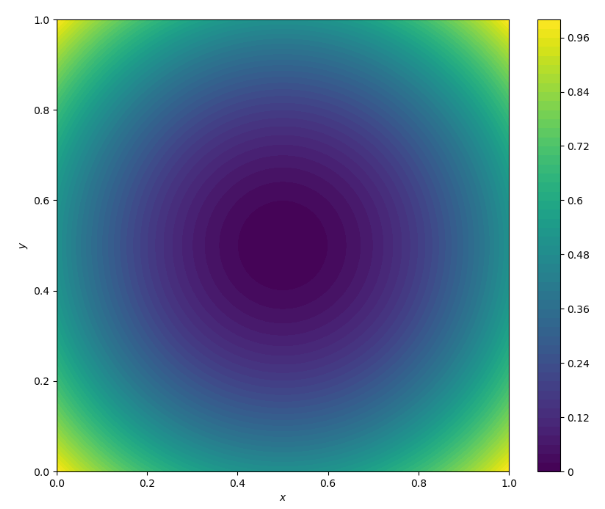
\includegraphics[width=\textwidth,height=0.85\textwidth]{Bonus1A.png}
		\caption{Fond non plat $A$}
	\end{subfigure}
	\begin{subfigure}{0.45\textwidth}
		\centering
		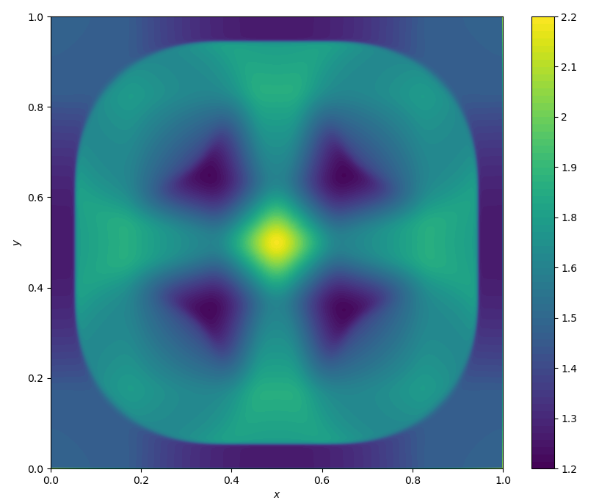
\includegraphics[width=\textwidth,height=0.85\textwidth]{Bonus1Aplush.png}
		\caption{Altitude d'eau finale $A+h$}
	\end{subfigure}
	\begin{subfigure}{0.32\textwidth}
		\centering
		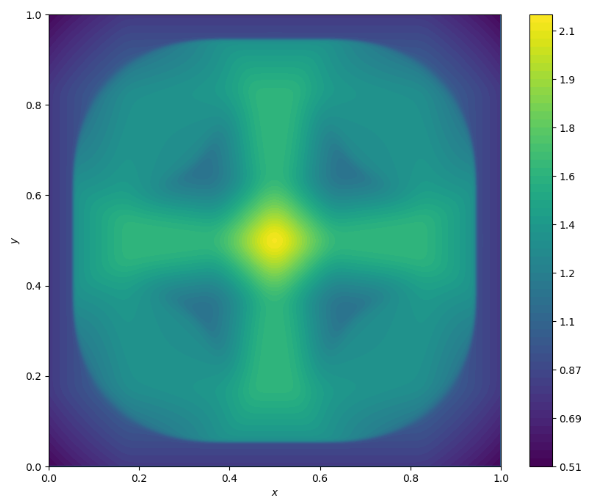
\includegraphics[width=\textwidth,height=0.85\textwidth]{Bonus1h.png}
		\caption{Hauteur d'eau finale}
		\label{fig:Bonus1h}
	\end{subfigure}
	\begin{subfigure}{0.32\textwidth}
		\centering
		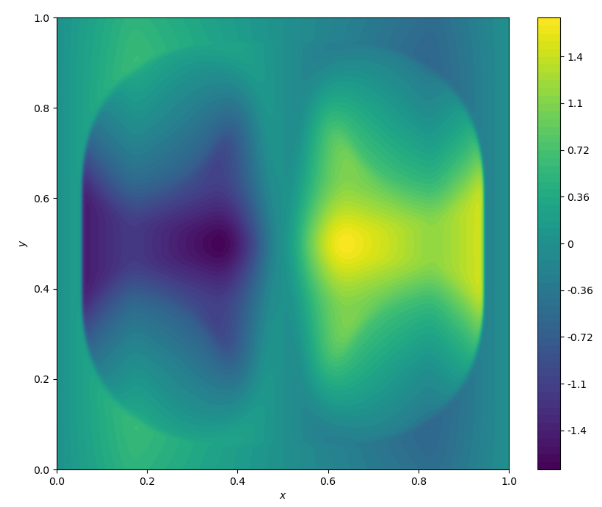
\includegraphics[width=\textwidth,height=0.85\textwidth]{Bonus1u.png}
		\caption{Vitesse suivant $x$ finale}
		\label{fig:Bonus1u}
	\end{subfigure}
	\begin{subfigure}{0.32\textwidth}
		\centering
		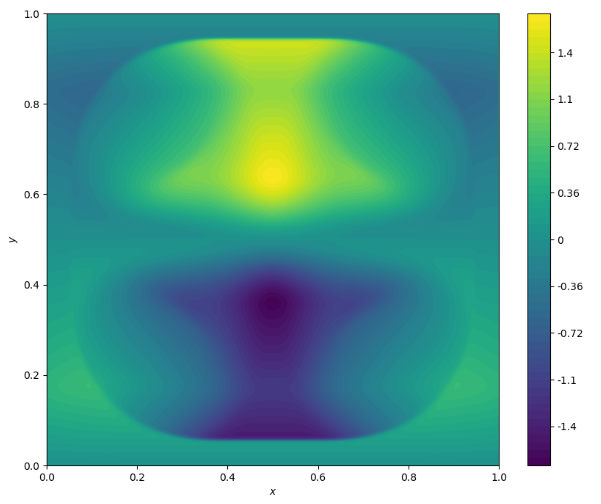
\includegraphics[width=\textwidth,height=0.85\textwidth]{Bonus1v.png}
		\caption{Vitesse suivant $y$ finale}
		\label{fig:Bonus1v}
	\end{subfigure}
	\caption{Illustration de la résolution du système de Saint-Venant sur un fond non plat. Comparé aux \cref{fig:Rusa3,fig:Riem3,fig:Muscl1}, on observe bien une tendance de l'eau sortie du barrage à y retourner.}
	\label{fig:Bonus1}
\end{figure}



\end{document}
